There are two basic classes / times for studies and evaluation (and many variants):
\begin{itemize}
\item \textbf{Formative}: At the beginning to inform about context and to study possible options
\item \textbf{Summative}: To judge on the impact of a HCI design.
A summative evaluation of a design might be a
formative one for the next step.
\end{itemize}
\textbf{Evaluation}: Iterative design \& evaluation is a continuous process that examines:
\begin{itemize}
\item Why to evaluate: to check users’ requirements and that they can use the product and they like it.
\item What to evaluate: a conceptual model, early prototypes of a new system and later, more complete prototypes.
\item Where to evaluate: in natural and laboratory settings.
\item When to evaluate: Formative: throughout design; Summative: finished products can be evaluated to collect information to inform new products.
\end{itemize}
\textbf{Usability}: The extent to which a product can be used by specified users to achieve specified goals with \textbf{effectiveness, efficiency and satisfaction} in a specified context of use.\\
 Over-arching usability principles: \textbf{Learnability, effectiveness, accommodation} for its intended user population.
 \begin{figure}[h!]
			\centering
			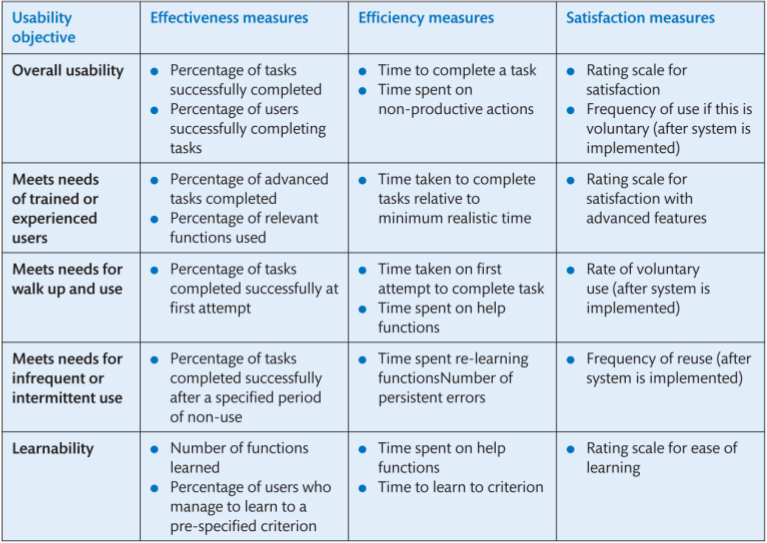
\includegraphics[width=\textwidth]{img/ch01_usab.png}
			\caption{What do we want to know -- Common usability metrics}
			\label{HAP}
		\end{figure} 
\textbf{Evaluation classes}:
\begin{itemize}
\item \textbf{Setting}:
\begin{itemize}
\item Controlled settings: Setting conditions are controlled; non-controllable conditions are measured; e.g. Lab experiments, living labs
\item Natural settings: Study in “everyday” and natural conditions that cannot be controlled; some, but not all non-controllable conditions can be measured; e.g. Field studies, in-the-wild studies
\end{itemize}
\item \textbf{Evaluation Time}:
\begin{itemize}
\item Inspective: Inspection / Evaluation while run of an experiment or while use
\item Retrospective: Evaluation after run of the experiment or after use
\item Short term
\item Long term
\end{itemize}
\item \textbf{Partner}:
\begin{itemize}
\item The user: Gives direct feedback e.g. for use; Best for gaining new insight into context (If its an experiment: called “subject”)
\item The expert: Allows for best practice information; Reported expert experience may require many users / test subjects to be collected
\end{itemize}
\item \textbf{Result type}:
\begin{itemize}
\item Subjective: Results cannot be directly compared between subjects
\item Objective Results can be directly compared between subjects (e.g. using statistics)
\item Quantitative: Results are numbers
\item Qualitative: Results are text
\end{itemize}
\end{itemize}
\textbf{Example Methods}:
\begin{itemize}
\item Inspective, End User Focused:
\begin{itemize}
\item Subjective Short Session: Think Aloud
\item Objective Short Session: Measurements of Workload, Interaction Process (e.g. Video Recording in User Setting / Usability Lab; Eye Gaze which is a quantitative/objective measure)
\item Subjective Long Session: Diary (Logging, asking questions from time to time e.g. through pop ups)
\end{itemize}
\item Inspective, Expert Focused: Cognitive Walk Through
\item Retrospective, End User Focused: Interviewing / Questionnaire
\end{itemize}
\textbf{Data Gathering -- Key Issues}
\begin{enumerate}
\item Setting goals: Decide how to analyze data once collected
\item Identifying participants: Decide who to gather data from
\item Relationship with participants: Clear and professional; Informed consent when appropriate
\item Triangulation: Look at data from more than one perspective; Collect more than one type of data, e.g. qualitative from experiments and qualitative from interviews.
\item Pilot studies: Small trial of main study
\end{enumerate}
\subsection{Data Gathering -- Interviews \& Questionnaires}
\textbf{Types of interviews}:
\begin{itemize}
\item \textbf{structured interviews}: pre-developed questions, strictly following the wording (e.g. introduction, purpose of the questionnaire); easy to carry out – but limited to the question set; more precise to evaluate
\item \textbf{semi-structured interviews}: structured part + “open” questions (“Tell me your ideas on ...”)
\item \textbf{unstructured interviews}: used e.g. when little background information is available; minimizes the influence of the questioner
\end{itemize}
Questionnaires: 
\begin{itemize}
\item Questions have orders (positive or negative, can be mixed)
\item Version needs to be adapted to population.
\item Instructions of use need to be clear.
\item No excess whitespace, not too long, no compound sentences or jargon.
\item frame: consent form, (monetary) compensation, time constraints, number of participants, introduction to scenario, scale type
\end{itemize}
Question and response format:
\begin{itemize}
\item Yes’ and ‘No’ checkboxes
\item Checkboxes that offer many options
\item Rating scales: Likert scales (5-point scale, \textit{strongly agree, agree, neutral, disagree, strongly disagree} --> quantitative result), semantic scales
\item Open-ended responses
\end{itemize}
Conducting the interview:
\begin{itemize}
\item contextual factors (light, noise...) should be kept constant, interviewer should provide a neutral attitude, interviewee might try to say what he thinks you want to hear --> questions to cross-check answers needed
\item[1.] Introduction: introduce yourself, explain the goals of the interview, reassure about the ethical issues, ask to record, present the informed consent form.
\item[2.] Warm-up: make first questions easy and non-threatening.
\item[3.] Main body: present questions in a logical order.
\item[4.] A cool-off period: include a few easy questions to defuse tension at the end.
\item[5.] Closure: thank interviewee, signal the end, e.g. switch recorder off.
\item documentation: notes, video taping, audio recording, photographs (always use visual impression)
\item interview can be enriched by props, e.g. prototype scenario
\item encouraging good responses: clarify purpose of study, promise anonymity, ensure questionnaire is well designed, Follow-up with emails/phone calls/letters, provide an incentive
--> 40\% response rate is good, 20\% is often acceptable
\end{itemize}
Standard Questionnaires in HCI:
\begin{itemize}
\item System Usability Scale (SUS)
\item NASA Task Load Index (TLX)
\item Questionnaire for User Interface Satisfaction (QUIS)
\item Computer System Usability Questionnaire (CSUQ)
\end{itemize}
\textbf{System Usability Scale (John Brooke, 1986 for Digital Equipment) }
\begin{itemize}
\item Quick and dirty subjective measurement of usability in terms of Effectiveness, Efficiency and Satisfaction
\item Used for hardware, software, mobile devices, websites, applications
\item Evaluation: Positive questions get a 0-4 rating, negative ones a 4-0 rating, points are added and multiplied by 2.5 -- good result if over 68 (max: 100)
\item Benefits: Very easy scale (Likert); Useful in small sample sizes with o.k. results; Validity o.k. (you see differences in bad and good design)
\item Restrictions: Score 0-100 (confusing, not a percentage); Not diagnostic, just to classify (no conclusion on specific problems possible)
\end{itemize}
\textbf{NASA Task Load Index}: Measures along 5 dimensions
\begin{itemize}
\item Mental demand: How mentally demanding was the task?
\item Physical demand: How physically demanding was the task
\item Temporal demand: How hurried or rushed was the pace of the task
\item Performance: How successful were you in accomplishing what you were asked to do
\item Effort: How hard did you have to work to accomplish your level of performance
\item Frustration: How insecure, discouraged, irritated, stressed and annoyed were you?
\end{itemize}
It consist of two steps:
\begin{itemize}
\item Step 1: The dimensions are scored on a 100 point scale, in increments of 5 (20 scale)
\item Step 2: User is then asked to perform 15 pair-wise comparisons to assess the weight for each of the measures (Asks the following question: “Which factor is the more
important contributor to work load for the task?”)
\item[-->] Second step reduces subjectivity greatly
\end{itemize}
Scoring procedure: For each dimension, sum the number of times it was selected as the leading pair wise factor. Divide this sum by 15 (the number of pairwise comparisons). Multiply this result by the score for each dimension. Sum the resulting dimension scores\\
Result: 0-100 score, weighted for dimensions considered important by the participant.\\
The optimum workload has to be determined case by case. Overload leads to poor performance due to stress. Underload leads to poor performance due to boredom.

\textbf{Online Questionnaires}:
\begin{itemize}
\item Advantages: Relatively easy and quick to distribute, Responses are usually received quickly, No copying and postage costs, Data can be collected in database for analysis, Time required for data analysis is reduced, Errors can be corrected easily
\item Problems: Sampling is problematic if population size is unknown, individuals cannot really be prevented from responding more than once, individuals have also been known to change questions in email questionnaires
\end{itemize}
Problems with interviews and questionnaires:
\begin{itemize}
\item retrospective, user may not remember (correctly) how he did everything
\item some aspects of interaction cannot be described verbally
\item user may try to answer how he feels is expected $\rightarrow$ observation shows how he actually does it, however: obtrusiveness (user is disturbed by the investigator's presence, time needed to decrease this effect)
\end{itemize}
\subsection{Data Gathering -- Observation}
Types of observation:
\begin{itemize}
\item Direct observation in controlled environments
\item Direct observation in the field: Structuring frameworks, Degree of participation (insider or outsider), Ethnography
\item Indirect observation: tracking users’ activities: Diaries, Experience Sampling Method (ESM), Interaction logging, Video and photographs collected remotely by drones or other equipment, web analytics
\item[$\rightarrow$] Video, audio, photos, notes are used to capture data in both types of observations
\end{itemize}

\textbf{Structuring frameworks}\\
1. Three easy-to-remember parts:
\begin{itemize}
\item The person: Who?
\item The place: Where?
\item The thing: What?
\end{itemize}
2. A more detailed framework (Robson, 2014):
\begin{itemize}
\item Space: What is the physical space like and how is it laid out?
\item Actors: What are the names and relevant details of the people involved?
\item Activities: What are the actors doing and why?
\item Objects: What physical objects are present, such as furniture
\item Acts: What are specific individual actions?
\item Events: Is what you observe part of a special event?
\item Time: What is the sequence of events?
\item Goals: What are the actors trying to accomplish?
\item Feelings: What is the mood of the group and of individuals?
\end{itemize}

\textbf{Materials that might be collected in observations}
\begin{itemize}
\item Activity or job descriptions.
\item Rules and procedures that govern particular activities.
\item Descriptions of activities observed.
\item Recordings of the talk taking place between parties.
\item Informal interviews with participants explaining the detail of observed activities.
\item Diagrams of the physical layout, including the position of artifacts.
\item Other information collected when observing activities: Photographs of artifacts (documents, diagrams, forms, computers, etc.), Videos of artifacts, Descriptions of artifacts, Workflow diagrams showing the sequential order of tasks, Process maps showing connections between activities
\end{itemize}
\subsubsection{Observation in a controlled environment}
\textbf{Think Aloud}
While using an application, a user is constantly explaining what he is thinking what he is doing. So-called cooperative usability evaluation (users work as co-evaluators), maximizing data from a simple testing session.\\
$\rightarrow$ The quality of the evaluation depends on 
\begin{itemize}
\item (as always) selection of test candidates: non-expert users preferred, all should have comparable visualization skills
\item appropriate preparation of the candidate
\item appropriate setting so that a natural usage can be guaranteed: quiet and comfortable, no interference from examiner, warm-up phase, as expectation free as possible
\end{itemize}
Think Aloud Session (c.f. table in Benyon p.280):
\begin{itemize}
\item preparation: explain system and setting (how test works, that system is tested and not the participant (!), that they should talk continuously) and expectation (that he should verbalize what he is doing and thinking about, just what comes to mind)
\item Recording device and experimenter should stay out of sight
\item Encourage participant to keep talking
\item Record video or audio, transcript
\item[$\rightarrow$] Qualitative, mostly subjective
\item[$\rightarrow$] Generalizations difficult
\item[$\rightarrow$] Psychological theories needed for interpretation
\item[$\rightarrow$] Helpful for intermediate formative design improvements
\end{itemize}

\subsubsection{Observation in the Field}
Laboratory-based usability testing and field studies can complement each other. One may use a field study to evaluate initial ideas and get early feedback, adapt the design accordingly and then perform a usability test do check specific design features. Then again a field study to see what happens when used in natural environment. Then some final design changes. 
\textbf{Ethnography}:
Ethnography is an interpretivist technique that includes participant observation and interviews.\\
The goal is to experience the participant and his context. Ethnographers immerse themselves in the culture that they study. A researcher's degree of participation can vary along a scale
from `outside' to `inside'. Analyzing video and data logs can be time-consuming. Collections of comments, incidents, and artifacts are made.
The co-operation of people being observed is required. Data analysis is continuous. Questions get refined as understanding grows. Reports usually contain examples.\\
Online-Ethnography (Netnography): Observing interactions in the information world. Interaction online differs from face-to-face! Virtual worlds have a persistence that physical worlds do not have. Ethical considerations and presentation of results are different.\\

\textbf{Living Labs}\\
\textbf{Ubicomp studies}:\\
Types:
\begin{itemize}
\item Studies of current behaviour -- What people doing now: better understanding of current use of technology, implications for future technology; open-ended questions; results=stories; starts from hours to weeks
\item Proof-of-concept studies -- Does my technology function in the real world: Validation of a (new) technology, often several days long
\item Experience studies -- How does using my prototype change people's behaviour or allow them to do new things: using the technology for a longer time (often several weeks), Wizard-of-Oz type studies (subjects interact with a computer system that subjects believe to be autonomous, but which is actually being operated or partially operated by an unseen human being)
\end{itemize}

\textbf{Study Design}
\begin{itemize}
\item start with a concrete research goal question that should be answered while study
\item Study design document:\\
-- Research question/hypothesis
-- Detailed participant profile
-- What will your participants do during the study: free or specific problem, do they use their own devices etc.
-- Detailed timeline description/How long will the study be
-- What data will you collect: quantitative (to \textit{compare} results) and qualitative (to better \textit{understand} results) data maximizes insight
-- Analysis method
-- Method of drawing conclusion/validating hypothesis
\end{itemize}

\subsubsection{Indirect observation methods}
Can be used in controlled and uncontrolled environments. Tracking users' activities using Diaries, Interaction logs, Web analytics. Need to be specific for specific application areas and settings.\\
\textbf{Logging}:\\
Select appropriate data to log at the right frequency, list specific questions that you expect to answer from the log data (best conduct small pilot study beforehand)
e.g. Web analytics: Typically focus on the number of web visitors and page views.\\

\textbf{Experience Sampling Methodology}:\\
Uses short questionnaires  that participant fill out at various points throughout the day (either randomly distributed, scheduled or at an event).\\

\textbf{Diaries}:\\
Participant has freedom when to enter information, but how to remind them to complete the diary?  

\subsubsection{General Considerations}
How long should the study be? Depends on:
\begin{itemize}
\item type of study: current behaviour, proof-of-concept, experience
\item novelty of system
\item effort from participants: measurement time needs to be restricted if it requires a lot
\item frequency of use: high frequency reduces required measurement time
\end{itemize}

Selecting Participants (should obviously not be from the designer group):
\begin{itemize}
\item Representation of Participants to the intended user group (e.g. the population, the worker,...)
\item Grouping of Participants: one or multiple groups? Group selection based on
\begin{itemize}
\item self-reported expertise (e.g. novice, intermediate, expert)
\item frequency of use (e.g. number of application use per day)
\item amount of experience (e.g. with working in a application domain, in days, month ..)
\item demographics (gender, age, location, etc.)
\item different activities the participants have to perform (e.g. each group only performs one type of work for a
program)
\end{itemize}
\item Data Sampling Strategy:
\begin{itemize}
\item Random Sampling: Everyone has equal probability to be selected as participant based on a list
\item Systematic Sampling: Based on predefined criteria, e.g. every 10th person entering the ECE Centre
\item Stratified Sampling: Additionally, it is important to select people reflecting the distribution in your intended user group. So you care e.g. that your final set contains 50\% male and 50\% female
\item Samples of convenience: Volunteer based. Must be adjusted to the wanted user group.
\end{itemize}
\end{itemize}

Sample size depends on acceptable error. 3-4 participants are enough to identify major problems, according to Nielsen on average 5 are enough in an early stage design (formative evaluation) to identify 75-80\% of usability problems.
Best perform a pre-test where participants have to first detect known usability issues. The average percentage $p$ of found usability issues over all the participants can be plugged into the formula $1-(1-p)^n$ to calculate the average amount of found issues for $n$ participants used.\\

Study design:
\begin{itemize}
\item Within subjects: One participant gets several task options, Results of task options are compared between the participant
\item Between subjects: Any subject gets the same task, compare how different users perform the task. Often users are grouped in categories beforehand (novice, expert...) Then user group performance is compared.
\item Mixed design studies are possible
\end{itemize}
Order of test tasks needs to be balanced across participants (at least of the tasks are somewhat related) $\rightarrow$ impossible if tasks depend on each other.

Interpreting the data: 
\begin{itemize}
\item Reliability: does the method produce the same results on separate occasions?
\item Validity: does the method measure what it is intended to measure? Internal Validity (certainty that you know the cause) vs. External Validity (result can be generalized)
\item Ecological validity: does the environment of the evaluation distort the results? Is the result transferable to a general environment?
\item Biases: Are there biases that distort the results?
\item Scope: How generalizable are the results?
\end{itemize}

\subsection{Inspections -- Evaluation without User}
\textbf{Types of Inspections}:
\begin{itemize}
\item Experts use their knowledge of users \& technology to review software usability. Expert critiques can be formal or informal.
\item Heuristic evaluation is a review guided by a set of heuristics.
\item Walkthroughs involve stepping through a pre-planned scenario noting potential problems.
\end{itemize}

\textbf{Heuristic Evaluation (Jacob Nielsen, 1990s}
\begin{itemize}
\item Visibility of system status.
\item Match between system and real world.
\item User control and freedom.
\item Consistency and standards.
\item Error prevention.
\item Recognition rather than recall.
\item Flexibility and efficiency of use.
\item Aesthetic and minimalist design.
\item Help users recognize, diagnose, recover from errors.
\item Help and documentation
\end{itemize}

Heuristics for websites focus on key criteria (Budd, 2007): Clarity, Minimize unnecessary complexity \& cognitive load, Provide users with context, Promote positive \& pleasurable user
experience.\\
Stages of heuristic evaluations:
\begin{enumerate}
\item Briefing session to tell experts what to do.
\item Evaluation period of 1-2 hours in which: Each expert works separately; one pass to get a feel for the product; a second pass to focus on specific features.
\item Debriefing session in which experts work together to prioritize problems.
\end{enumerate}

Advantages: Few ethical \& practical issues to consider because users not involved.\\
Disadvantages: Can be difficult \& expensive to find experts as they need to have knowledge of application domain and users. Important problems may get missed; Many trivial problems are often identified; Experts have biases.

\textbf{Cognitive Walkthrough}:\\
Focus on ease of learning. Designer presents an aspect of the design \& usage scenarios. Expert is told the assumptions about user population, context of use, task details. One or more experts walk through the design prototype with the scenario. Experts are guided by 3 questions:
\begin{itemize}
\item Will the correct action be sufficiently evident to the user?
\item Will the user notice that the correct action is available?
\item Will the user associate and interpret the response from the action correctly?
\end{itemize}

Variation -- Pluralistic Walkthrough: Experts work separately, then discuss. Walkthroughs are focused so are suitable for evaluating small parts of a product. \\

\textbf{Predicive models}:
Provide a way of evaluating products or designs without directly involving users and are less expensive than user testing. Their usefulness limited to systems with predictable
tasks - e.g. telephone answering systems, mobiles, cell and smart phones. They are based on expert error-free behavior. Fitts' law predicts that the time required to rapidly move to a target area is a function of the ratio between the distance to the target and the width of the target. Thus, it applies to clearly defined tasks with limited key presses, such as data entry and smart phone use.

\textbf{Workload Assessment}
Criteria for Creating an Measure of Mental Workload:
\begin{itemize}
\item Sensitivity: index must be sensitive to changes in task difficulty or resource demand
\item Selectivity: index should NOT be sensitive to changes unrelated to resource demands
\item Diagnosticity: index should indicate not just that workload is varying but the cause of variation
\item (Un)Obtrusiveness: an index should not interfere with or contaminate the primary task being assessed
\item Reliability (Reproducibility): index should produce the same estimate for a given task and operator
\item Bandwidth: the index should respond to high-frequency (quick) changes in workload
\end{itemize}
Workload can be assessed via performance metrics (time, speed, strength) or physiologic metrics (heart rate, respiration, oxygen uptake). 
Tool: NASA TLX